
\documentclass[11pt,a4paper]{article}

\usepackage[utf8]{inputenc}
\usepackage[T1]{fontenc}
\usepackage{lmodern}
\usepackage{geometry}
\usepackage{amsmath,amssymb,mathtools}
\usepackage{booktabs}
\usepackage{array}
\usepackage{enumitem}
\usepackage{hyperref}
\usepackage{xcolor}
\usepackage{tikz}
\usepackage{pgfplots}
\usepackage{float}
\usepackage{caption}
\usepackage{microtype}
\usepackage{graphicx}
\usepackage{tabularx}

\usetikzlibrary{arrows.meta,positioning,shapes.geometric,fit,calc}
\pgfplotsset{compat=1.18}

\geometry{margin=0.85in}
\hypersetup{colorlinks=true,linkcolor=blue!60!black,citecolor=blue!60!black,urlcolor=blue!60!black}
\setlength{\parindent}{0pt}
\setlength{\parskip}{6pt}

\tikzset{
 block/.style={rectangle,rounded corners=3pt,draw=black!60,minimum width=3.1cm,minimum height=0.85cm,align=center,fill=gray!7},
 important/.style={rectangle,rounded corners=3pt,draw=black!70,minimum width=3.4cm,minimum height=0.95cm,align=center,fill=blue!7},
 arrow/.style={-{Latex[length=2.5mm]},thick}
}

\title{\textbf{Gap-Aware Retrieval (GAR)}\\[4pt]\large A Gap-Aware Retrieval Algorithm for Iterative Retrieval-Augmented Generation}
\author{}
\date{}

\begin{document}
\maketitle

\begin{abstract}
Retrieval-Augmented Generation (RAG) systems usually select documents according to their relevance to a query. This can be insufficient for complex, multi-step questions because a document can be highly related to the topic while still failing to provide the information that is currently missing. This project proposes \textbf{Gap-Aware Retrieval (GAR)}, a retrieval algorithm that explicitly considers the current information gap and previously collected evidence when selecting documents.

MIGRES is used as the base system. MIGRES is a Missing Information Guided Retrieve-Extraction-Solving framework in which missing information is used to guide later retrieval. Its reported baseline uses BM25. GAR therefore replaces the document retrieval component while the remaining MIGRES pipeline is kept fixed as far as possible. The project compares MIGRES+GAR against MIGRES+BM25, DPR, Contriever, ColBERTv2, and SPLADE.

GAR is formulated using three proposed signals: gap relevance, gap coverage, and evidence novelty. The project evaluates retrieval quality, downstream answer quality, efficiency, ablations, and statistical significance. The main datasets are the six datasets reported in the MIGRES evaluation: WikiHop, HotpotQA, MuSiQue, Natural Questions, TriviaQA, and StrategyQA. The current formulation is a research proposal motivated by existing literature; a formal novelty claim requires a final literature and implementation check.
\end{abstract}

\section{Introduction}

Retrieval is a central component of modern Retrieval-Augmented Generation systems. A retriever is responsible for selecting a small set of documents from a large corpus so that a downstream model can use them to answer a question. A common approach is to rank documents according to their similarity to the query.

This approach is useful, but it has a weakness in iterative information-seeking tasks. After one retrieval step, the system may already know part of the answer. The next retrieval step should therefore not simply find documents that are relevant to the original question. It should find documents that provide the information that is still missing.

For example, consider the question ``Why did Company X's revenue increase?'' Suppose the system already knows that the revenue increased by 30 percent. A conventional retriever can repeatedly return documents mentioning the 30 percent increase. These documents are relevant to the topic, but they do not necessarily answer the remaining question: why did the increase happen?

This project studies whether retrieval can be improved by explicitly using the current information gap and the evidence already collected. The proposed algorithm is called Gap-Aware Retrieval (GAR).


\section{About the Baseline Paper: MIGRES}

MIGRES is the base system for this project. The MIGRES framework uses missing information to guide retrieval in an iterative process. Its Retrieval Module contains query generation, retrieval, and knowledge filtering components.

The important experimental idea is to change the retrieval component while leaving the rest of MIGRES fixed.

\begin{center}
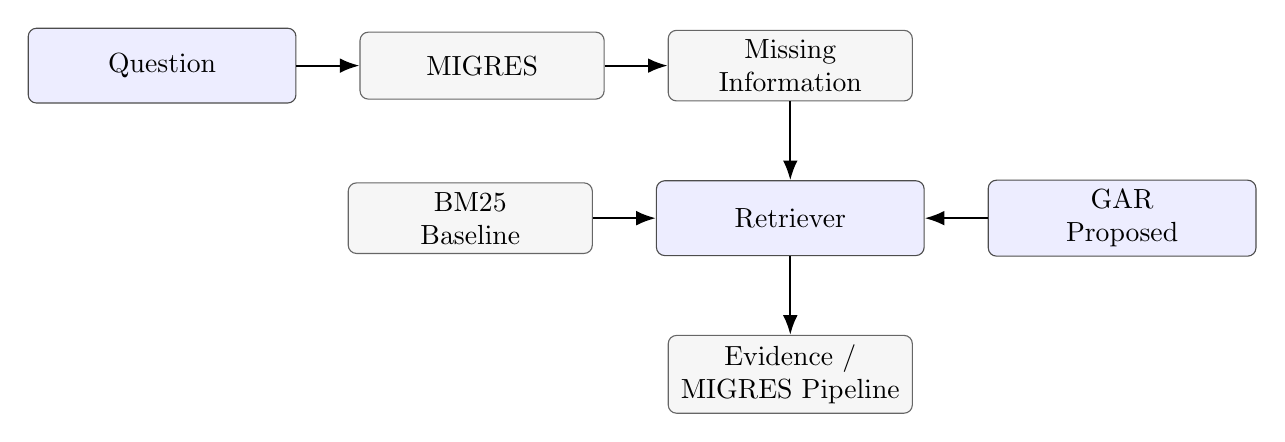
\begin{tikzpicture}[node distance=10mm and 8mm]
\node[important] (q) {Question};
\node[block,right=of q] (m) {MIGRES};
\node[block,right=of m] (g) {Missing\\Information};
\node[important,below=of g] (r) {Retriever};
\node[block,left=of r] (b) {BM25\\Baseline};
\node[important,right=of r] (gar) {GAR\\Proposed};
\node[block,below=of r] (e) {Evidence /\\MIGRES Pipeline};

\draw[arrow] (q) -- (m);
\draw[arrow] (m) -- (g);
\draw[arrow] (g) -- (r);
\draw[arrow] (b) -- (r);
\draw[arrow] (gar) -- (r);
\draw[arrow] (r) -- (e);
\end{tikzpicture}
\end{center}

\captionof{figure}{MIGRES is the fixed experimental framework; the retriever is the main experimental variable.}

The original system is:

\[
\text{MIGRES}+\text{BM25}.
\]

Our proposed system is:

\[
\text{MIGRES}+\text{GAR}.
\]

The iterative loop remains part of MIGRES:

\[
\text{Question}
\rightarrow
\text{Retrieval}
\rightarrow
\text{Evidence}
\rightarrow
\text{Missing Information}
\rightarrow
\text{Retrieval}.
\]

GAR is the retrieval method used at the retrieval stage.


\section{What Is an Information Retrieval Algorithm?}

Information Retrieval (IR) is the task of finding useful information from a large collection of information. In our project, the collection is a document corpus and the input is a question or query.

A simple retrieval system can be written as:

\[
q + D \longrightarrow d_1,d_2,\ldots,d_k
\]

where $q$ is the query, $D$ is the document collection, and the output is a ranked list of the best documents.

The important part is the scoring function. A retriever gives each candidate document a score and returns the documents with the highest scores. Different retrieval algorithms use different ways to calculate that score.

\subsection{BM25}

BM25 is a traditional sparse retrieval method. It mainly uses word matching between the query and document. It also considers how often a word appears, how common the word is in the whole collection, and document length. BM25 is our main baseline because MIGRES uses it in its reported retrieval setup.

\subsection{DPR}

Dense Passage Retrieval (DPR) represents questions and passages as dense vectors. It then compares the vectors to find semantically related passages \cite{dpr}. DPR is a strong dense retrieval baseline.

\subsection{Contriever}

Contriever is an unsupervised dense retrieval method. It learns useful representations without the same supervised retrieval training setup used by DPR \cite{contriever}. It gives us a different dense-retrieval baseline.

\subsection{ColBERTv2}

ColBERTv2 uses late interaction. Instead of representing the whole document and question using only one vector, it keeps token-level representations and compares them efficiently. This makes it a useful comparison with both sparse and single-vector dense retrieval \cite{colbert}.

\subsection{SPLADE}

SPLADE is a neural sparse retrieval method. It creates sparse representations while using a neural model to expand and weight useful terms. It combines some benefits of neural representation learning with efficient sparse retrieval \cite{splade}.

Therefore, the main retrieval methods in our experiment are:

\[
\boxed{
\text{BM25},\ \text{DPR},\ \text{Contriever},\ \text{ColBERTv2},\ \text{SPLADE},\ \text{GAR}
}
\]

GAR is different from the other methods because its score explicitly uses the current information gap and already collected evidence.


\section{How We Made the GAR Equation}

The equation is not copied from one paper. It is a simple combination of three ideas that already exist in the literature. We use those ideas as building blocks and then define one retrieval score for this project.

First, MIGRES gives us the idea of an \textbf{information gap}. MIGRES asks what information is still missing after the system has already collected some evidence \cite{migres}. We use this idea through the variable $G$.

Second, Yadav, Bethard, and Surdeanu proposed an iterative evidence retrieval method that focuses later retrieval on terms that are not already covered by the current evidence. Their paper also defines a coverage measure \cite{air}. We use the general idea of \textbf{coverage of what is still missing}. We do not copy their exact formula.

Third, the Relevant Information Gain paper argues that retrieved information should be relevant but should also avoid unnecessary repetition. It proposes an information-gain objective so that useful diversity can appear among retrieved passages \cite{rig}. We use this idea through the \textbf{novelty} term. Again, our equation is not the same as the equation in that paper.

Therefore, the three ideas become:

\begin{center}
\begin{tabular}{lll}
\toprule
\textbf{Source} & \textbf{Idea used} & \textbf{GAR term}\\
\midrule
MIGRES & What information is missing? & $G$\\
Yadav et al. & How much missing information is covered? & $C(d,G)$\\
Relevant Information Gain & How much useful new information is added? & $N(d,E)$\\
\bottomrule\end{tabular}
\end{center}

We then keep the normal question-document relevance idea and combine all three signals into one score:

\[
\boxed{
S(d\mid q,E,G)=\alpha R(d,q,G)+\beta C(d,G)+\gamma N(d,E)
}
\]

In plain English, the equation says:

\begin{quote}
\textbf{Choose documents that are relevant, that help fill the current gap, and that add useful information that we do not already have.}
\end{quote}

This is the proposed GAR model. Its novelty should be stated carefully until the final literature review confirms that no previous paper uses the same complete formulation.


\section{What Exactly Is GAR?}

\subsection{What GAR Is}

GAR is a retrieval algorithm based on the idea that the usefulness of a document depends on the current state of the information need.

Instead of using only:

\[
\operatorname{sim}(q,d),
\]

GAR considers three questions:

\begin{enumerate}[leftmargin=1.5em]
\item Is the document relevant to the question and the current information gap?
\item Does the document cover information that is currently missing?
\item Does the document provide information that is not already present in the collected evidence?
\end{enumerate}

The algorithm therefore attempts to distinguish between \emph{relevant information} and \emph{useful new information}.

\subsection{How GAR Works}

The input to GAR is:

\[
(q,E,G,D),
\]

where $q$ is the original question, $E$ is previously collected evidence, $G$ is the current information gap, and $D$ is the document corpus.

GAR scores candidate documents. The highest-scoring documents are returned.

\begin{center}
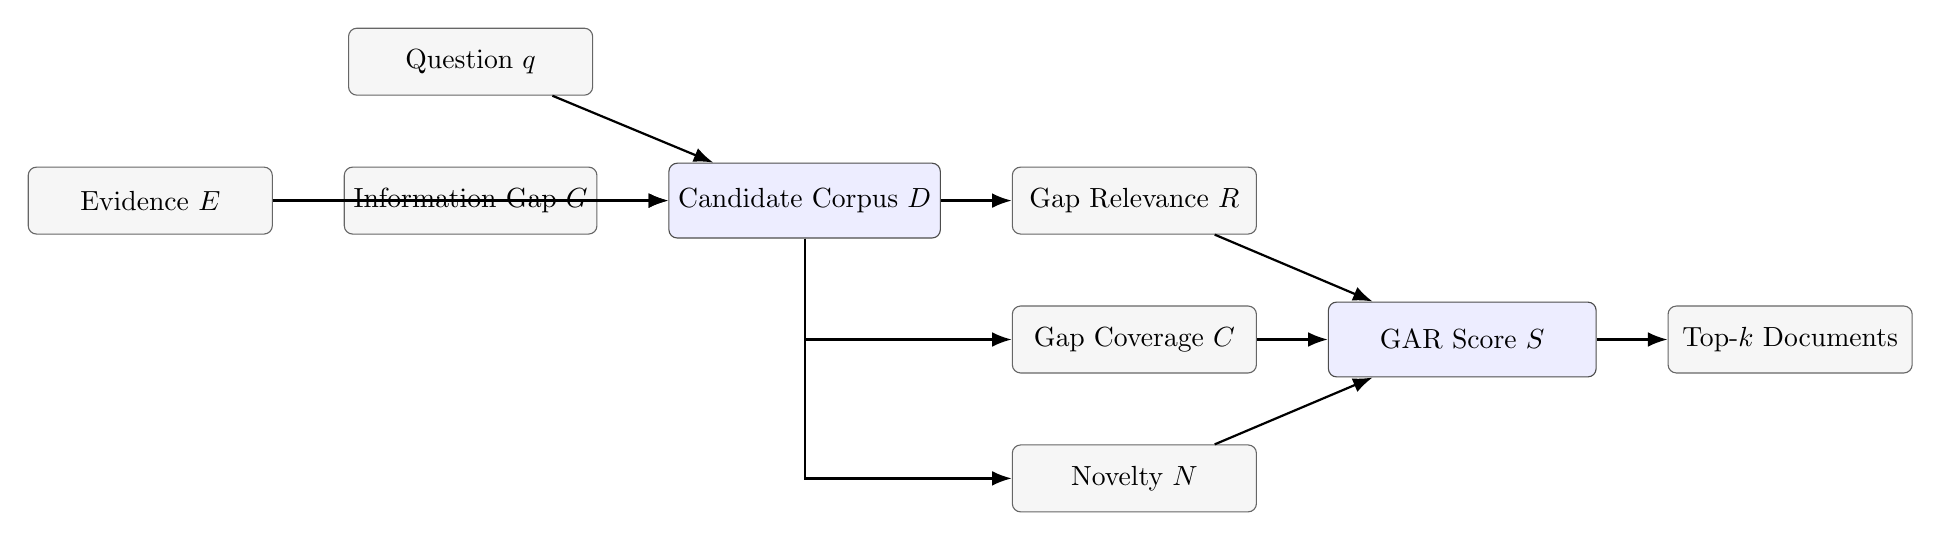
\begin{tikzpicture}[node distance=9mm and 9mm]
\node[block] (q) {Question $q$};
\node[block,below=of q] (g) {Information Gap $G$};
\node[block,left=of g] (e) {Evidence $E$};
\node[important,right=of g] (d) {Candidate Corpus $D$};
\node[block,right=of d] (r) {Gap Relevance $R$};
\node[block,below=of r] (c) {Gap Coverage $C$};
\node[block,below=of c] (n) {Novelty $N$};
\node[important,right=of c] (s) {GAR Score $S$};
\node[block,right=of s] (t) {Top-$k$ Documents};

\draw[arrow] (q) -- (d);
\draw[arrow] (g) -- (d);
\draw[arrow] (e) -- (d);
\draw[arrow] (d) -- (r);
\draw[arrow] (d) |- (c);
\draw[arrow] (d) |- (n);
\draw[arrow] (r) -- (s);
\draw[arrow] (c) -- (s);
\draw[arrow] (n) -- (s);
\draw[arrow] (s) -- (t);
\end{tikzpicture}
\end{center}

\captionof{figure}{Conceptual architecture of the proposed Gap-Aware Retrieval algorithm.}

\subsection{Why It Can Be Useful}

GAR is designed for settings where the system's information need changes after evidence is collected. Potential applications include multi-hop question answering, research-oriented RAG, evidence retrieval, OSINT-style information gathering, and other iterative information-seeking systems.

GAR does not require a separate agent or a new large language model. The surrounding system may supply the information gap and evidence state. GAR then performs document selection.

\subsection{Advantages}

The intended advantages are that GAR is modular, interpretable, and compatible with existing retrieval pipelines. Its score exposes why a document was preferred: relevance, coverage, and novelty.

Another advantage is that it can be evaluated without creating a new benchmark. Existing datasets with supporting evidence can provide retrieval ground truth.

\subsection{Disadvantages and Risks}

The main risk is that novelty can reward documents that are different but irrelevant. Therefore novelty must not be used by itself.

Another challenge is operationalizing gap coverage without making the system too expensive. The project should avoid requiring a separate LLM call for every candidate document if a cheaper representation or matching mechanism can be used.

The weighting parameters can also change performance. They therefore need to be selected using validation data or learned in a controlled way.

Finally, if GAR uses BM25 to retrieve a candidate pool and only reranks that pool, it becomes a reranker rather than a complete first-stage retriever. The implementation must clearly define whether GAR itself retrieves from the corpus or only reranks externally generated candidates.


\section{Mathematical Formulation}

Let:

\begin{align}
q &= \text{original question},\\
E &= \text{evidence already collected},\\
G &= \text{current information gap},\\
d &= \text{candidate document},\\
D &= \text{document corpus}.
\end{align}

The proposed GAR score is:

\[
\boxed{
S(d\mid q,E,G)
=
\alpha R(d,q,G)
+
\beta C(d,G)
+
\gamma N(d,E)
}
\tag{1}
\]

The retriever returns:

\[
\boxed{
TopK =
\operatorname{TopK}_{d\in D}
S(d\mid q,E,G)
}
\tag{2}
\]

Equation (1) contains three terms: gap relevance, gap coverage, and evidence novelty.

\subsection{Gap Relevance}

Gap relevance is:

\[
\boxed{
R(d,q,G)
=
\lambda\operatorname{sim}(d,q)
+
(1-\lambda)\operatorname{sim}(d,G)
}
\tag{3}
\]

The first similarity measures how related the document is to the original question. The second measures how related it is to the information gap.

The parameter $\lambda$ controls the balance.

If $\lambda$ is high, the original question receives more weight. If $\lambda$ is low, the information gap receives more weight.

Similarity can be implemented using cosine similarity:

\[
\boxed{
\operatorname{sim}(\mathbf{x},\mathbf{y})
=
\frac{\mathbf{x}^{T}\mathbf{y}}
{\|\mathbf{x}\|\|\mathbf{y}\|}
}
\tag{4}
\]

For example, a document explaining why revenue increased should have higher similarity to a gap such as ``cause of revenue increase'' than a document that only discusses the company's stock price.

\subsection{Gap Coverage}

The second component is:

\[
C(d,G).
\]

The information gap can contain several requirements:

\[
\boxed{
G=\{g_1,g_2,\ldots,g_k\}
}
\tag{5}
\]

A proposed weighted coverage score is:

\[
\boxed{
C(d,G)
=
\frac{
\sum_{i=1}^{k}w_i c(d,g_i)
}{
\sum_{i=1}^{k}w_i
}
}
\tag{6}
\]

Here, $c(d,g_i)$ measures how well document $d$ covers requirement $g_i$, while $w_i$ represents the importance of that requirement.

For example, suppose:

\[
G=
\{
\text{cause of revenue increase},
\text{supporting evidence}
\}.
\]

A document that only repeats the revenue number has low coverage. A document that explains the cause and provides evidence has higher coverage.

This coverage formulation is a proposed component of GAR. It should be treated as part of our research contribution rather than as a formula directly copied from MIGRES.

\subsection{Evidence Novelty}

The third component is:

\[
N(d,E).
\]

A simple proposed formulation is:

\[
\boxed{
N(d,E)
=
1-
\max_{e\in E}\operatorname{sim}(d,e)
}
\tag{7}
\]

The purpose is to reduce the score of documents that repeat information already collected.

If a candidate is nearly identical to an existing evidence item:

\[
\operatorname{sim}(d,e)\approx1,
\]

then:

\[
N(d,E)\approx0.
\]

If it is substantially different:

\[
\operatorname{sim}(d,e)\approx0,
\]

then:

\[
N(d,E)\approx1.
\]

For the first retrieval step, where $E=\emptyset$, the implementation must define a neutral/default novelty value.

\subsection{Meaning of the Greek Letters}

The Greek letters are weights:

\[
\alpha=\text{weight of gap relevance},
\]

\[
\beta=\text{weight of gap coverage},
\]

\[
\gamma=\text{weight of evidence novelty}.
\]

A convenient constraint is:

\[
\boxed{
\alpha+\beta+\gamma=1,
\qquad
\alpha,\beta,\gamma\geq0.
}
\tag{8}
\]

The parameter $\lambda$ in Equation (3) is also a weight:

\[
0\leq\lambda\leq1.
\]

It determines how much importance is given to the original question versus the information gap.

These parameters should be determined using validation experiments rather than chosen solely by intuition.

\subsection{Numerical Example}

Suppose a candidate document receives:

\[
R=0.80,\qquad C=0.90,\qquad N=0.60.
\]

Let:

\[
\alpha=0.30,\qquad
\beta=0.50,\qquad
\gamma=0.20.
\]

Then:

\begin{align*}
S(d)
&=0.30(0.80)+0.50(0.90)+0.20(0.60)\\
&=0.24+0.45+0.12\\
&=0.81.
\end{align*}

Thus:

\[
\boxed{S(d)=0.81}.
\]

The same calculation is performed for candidate documents. The highest-scoring candidates are returned.


\section{MIGRES System for Our Project}

MIGRES is the base system for this project. The MIGRES framework uses missing information to guide retrieval in an iterative process. Its Retrieval Module contains query generation, retrieval, and knowledge filtering components.

The important experimental idea is to change the retrieval component while leaving the rest of MIGRES fixed.

\begin{center}
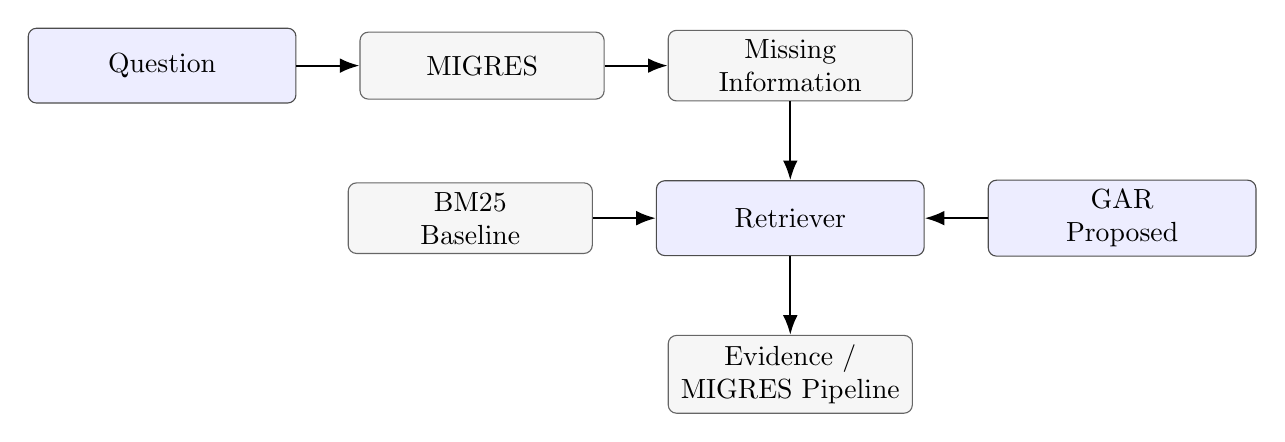
\begin{tikzpicture}[node distance=10mm and 8mm]
\node[important] (q) {Question};
\node[block,right=of q] (m) {MIGRES};
\node[block,right=of m] (g) {Missing\\Information};
\node[important,below=of g] (r) {Retriever};
\node[block,left=of r] (b) {BM25\\Baseline};
\node[important,right=of r] (gar) {GAR\\Proposed};
\node[block,below=of r] (e) {Evidence /\\MIGRES Pipeline};

\draw[arrow] (q) -- (m);
\draw[arrow] (m) -- (g);
\draw[arrow] (g) -- (r);
\draw[arrow] (b) -- (r);
\draw[arrow] (gar) -- (r);
\draw[arrow] (r) -- (e);
\end{tikzpicture}
\end{center}

\captionof{figure}{MIGRES is the fixed experimental framework; the retriever is the main experimental variable.}

The original system is:

\[
\text{MIGRES}+\text{BM25}.
\]

Our proposed system is:

\[
\text{MIGRES}+\text{GAR}.
\]

The iterative loop remains part of MIGRES:

\[
\text{Question}
\rightarrow
\text{Retrieval}
\rightarrow
\text{Evidence}
\rightarrow
\text{Missing Information}
\rightarrow
\text{Retrieval}.
\]

GAR is the retrieval method used at the retrieval stage.


\section{How the Datasets Are Used}

We do not need to collect a new dataset for the first version of this project. The six datasets used by MIGRES are already public benchmarks with published papers. They provide questions, evidence, answers, or supporting annotations that can be used for evaluation.

The dataset is used in two different ways. During retrieval, GAR sees only the information that a real system is allowed to see: the question, current evidence, information gap, and document corpus. During evaluation, the benchmark's supporting evidence or answer annotations are used as ground truth. GAR must not see the ground-truth evidence while retrieving.

For development, HotpotQA FullWiki is a sensible first dataset because it contains supporting facts and a large Wikipedia retrieval setting. After the implementation works, the remaining MIGRES datasets can be used to test whether the method generalizes.


\section{Datasets}

\subsection{Dataset Selection}

MIGRES's main evaluation reports six datasets:

\begin{enumerate}[leftmargin=1.5em]
\item WikiHop,
\item HotpotQA,
\item MuSiQue,
\item Natural Questions (NQ),
\item TriviaQA,
\item StrategyQA.
\end{enumerate}

These datasets cover different forms of open-domain, multi-hop, and reasoning-oriented question answering.

The initial development should use HotpotQA FullWiki because it provides explicit supporting facts and a full-corpus retrieval setting. After the implementation is stable, the other MIGRES datasets can be used for generalization.

No new dataset needs to be collected for the initial project.

\subsection{WikiHop}

WikiHop is a multi-hop reading-comprehension dataset constructed to require information to be combined across documents. It contains approximately 51K examples in the published benchmark.

Its relevance to GAR is that the system must identify useful documents from candidate evidence rather than relying on one isolated passage.

Dataset paper:
\url{https://aclanthology.org/Q18-1021/}

\subsection{HotpotQA}

HotpotQA contains approximately 113K Wikipedia-based question-answer pairs. It is particularly useful for retrieval research because it contains sentence-level supporting facts and multi-hop questions.

Two commonly used settings are the distractor setting and the FullWiki setting. FullWiki is more appropriate for a first-stage retrieval experiment because the retriever searches the larger processed Wikipedia corpus.

The official HotpotQA resources provide data and a processed Wikipedia corpus, and the repository supports replacing retrieval with a custom IR system.

Dataset paper:
\url{https://aclanthology.org/D18-1259/}

Official resources:
\url{https://hotpotqa.github.io/}

\subsection{MuSiQue}

MuSiQue contains approximately 25K questions designed around compositional multi-hop reasoning. The benchmark focuses on connecting multiple reasoning steps instead of simply retrieving unrelated evidence.

This is relevant to GAR because a retrieval algorithm should be able to support different information needs across multiple steps.

Dataset paper:
\url{https://aclanthology.org/2022.tacl-1.31/}

Official repository:
\url{https://github.com/StonyBrookNLP/musique}

\subsection{Natural Questions}

Natural Questions is based on real, anonymized, aggregated questions issued to Google Search. Annotators were shown Wikipedia pages and identified long answers and short answers where applicable.

The released dataset contains 307,373 training examples, 7,830 development examples, and 7,842 test examples.

NQ is useful because it is not designed exclusively as a multi-hop benchmark. It therefore helps test whether the gap-aware idea remains useful in a broader open-domain setting.

Dataset paper:
\url{https://aclanthology.org/Q19-1026/}

Official data:
\url{https://ai.google.com/research/NaturalQuestions/download}

\subsection{TriviaQA}

TriviaQA contains approximately 95K question-answer pairs and more than 650K question-answer-evidence triples in its published release.

Questions were authored by trivia enthusiasts, and evidence documents were gathered independently. This makes it useful for studying retrieval from heterogeneous evidence.

Dataset paper:
\url{https://aclanthology.org/P17-1147/}

Official resources:
\url{https://nlp.cs.washington.edu/triviaqa/}

\subsection{StrategyQA}

StrategyQA contains 2,780 verified questions. It focuses on implicit multi-step reasoning. The dataset includes reasoning decompositions and evidence paragraphs associated with reasoning steps.

This makes StrategyQA useful for testing retrieval when the required reasoning path is not explicitly written in the question.

Dataset paper:
\url{https://aclanthology.org/2021.tacl-1.21/}

Official resources:
\url{https://allenai.org/data/strategyqa}

\subsection{Dataset Summary}

\begin{center}
\small
\begin{tabular}{p{2.8cm}p{3.2cm}p{8.0cm}}
\toprule
\textbf{Dataset} & \textbf{Approx. scale} & \textbf{Important feature}\\
\midrule
WikiHop & 51K examples & Multi-document, multi-hop reasoning.\\
HotpotQA & 113K QA pairs & Multi-hop questions and sentence-level supporting facts.\\
MuSiQue & 25K questions & Compositional 2--4 hop reasoning.\\
NQ & 307,373 train; 7,830 dev; 7,842 test & Real search questions with Wikipedia evidence.\\
TriviaQA & 95K QA pairs; $>$650K evidence triples & Heterogeneous evidence and open-domain QA.\\
StrategyQA & 2,780 verified questions & Implicit reasoning with evidence for reasoning steps.\\
\bottomrule
\end{tabular}
\end{center}

\captionof{table}{Published dataset characteristics. Exact numbers can vary by release, preprocessing, and split. The exact files loaded in the experiment must be taken from the MIGRES repository configuration.}

\begin{figure}[H]
\centering
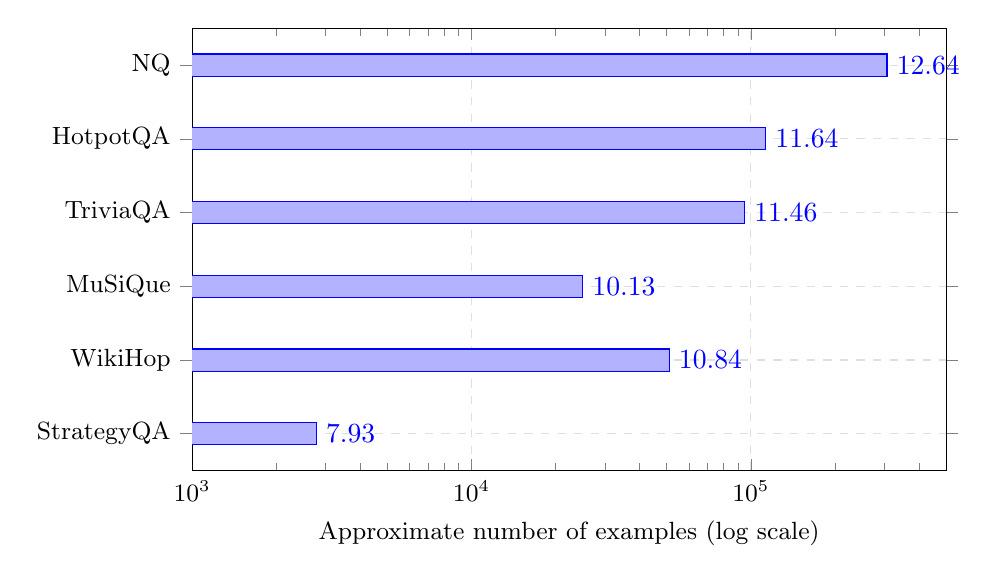
\begin{tikzpicture}
\begin{axis}[
xbar,
width=0.92\textwidth,
height=7.2cm,
xmode=log,
xmin=1000,
xmax=500000,
symbolic y coords={StrategyQA,WikiHop,MuSiQue,TriviaQA,HotpotQA,NQ},
ytick=data,
xlabel={Approximate number of examples (log scale)},
nodes near coords,
nodes near coords align={horizontal},
bar width=8pt,
grid=major,
grid style={dashed,gray!25},
tick label style={font=\small},
label style={font=\small}
]
\addplot coordinates {
(2780,StrategyQA)
(51000,WikiHop)
(25000,MuSiQue)
(95000,TriviaQA)
(113000,HotpotQA)
(307373,NQ)
};
\end{axis}
\end{tikzpicture}
\caption{Approximate published dataset sizes. The logarithmic axis is used because the dataset sizes differ substantially.}
\end{figure}


\section{How We Will Use GAR with MIGRES}

The implementation will be controlled. First, we reproduce the original MIGRES system with BM25. This gives us a working baseline. Next, we find the exact retrieval interface in the MIGRES code. GAR is then implemented with the same input-output role as the original retriever.

The main comparison is:

\[
\boxed{\text{MIGRES+BM25}\quad vs.\quad\text{MIGRES+GAR}}
\]

After that, we add the other retrieval baselines:

\[
\text{MIGRES+BM25},\quad
\text{MIGRES+DPR},\quad
\text{MIGRES+Contriever},
\]
\[
\text{MIGRES+ColBERTv2},\quad
\text{MIGRES+SPLADE},\quad
\text{MIGRES+GAR}.
\]

The same dataset, corpus, questions, and MIGRES settings should be used as far as possible. This makes the retrieval method the main changing variable.

A very important implementation point is the difference between a retriever and a reranker. A complete GAR retriever should search the corpus itself:

\[
(q,E,G,D)\rightarrow GAR\rightarrow TopK.
\]

If GAR first receives a BM25 candidate list and only reorders those documents, then it is a reranker. That is a different research claim. Because this project is about retrieval, we should aim for the first design.


\section{Experimental and Evaluation Plan}

The experiment should be controlled so that the retrieval algorithm is the main variable.

The systems are:

\begin{center}
\begin{tabular}{ll}
\toprule
\textbf{System} & \textbf{Retriever}\\
\midrule
MIGRES + BM25 & BM25\\
MIGRES + DPR & DPR\\
MIGRES + Contriever & Contriever\\
MIGRES + ColBERTv2 & ColBERTv2\\
MIGRES + SPLADE & SPLADE\\
MIGRES + GAR & Proposed method\\
\bottomrule
\end{tabular}
\end{center}

The same dataset, corpus, question set, MIGRES modules, stopping conditions, and evaluation procedure should be used wherever possible.

\subsection{Retrieval Metrics}

\textbf{Recall@k} measures whether required evidence appears in the top-$k$ retrieved documents.

\[
Recall@k=
\frac{\text{relevant evidence retrieved in top }k}
{\text{total relevant evidence}}.
\]

\textbf{Precision@k} measures how much of the top-$k$ retrieval is relevant:

\[
Precision@k=
\frac{\text{relevant documents in top }k}{k}.
\]

\textbf{MRR} measures how early the first relevant document appears:

\[
MRR=
\frac{1}{N}
\sum_{i=1}^{N}
\frac{1}{rank_i}.
\]

\textbf{nDCG} can be used when relevance is graded rather than binary.

Because GAR is specifically gap-aware, we should also report an evidence-coverage measure where the dataset's annotations make this possible.

\subsection{Downstream Metrics}

The retrieval results should also be evaluated through the downstream MIGRES task. Depending on the dataset and available annotations, this can include Exact Match, F1, answer accuracy, and evidence/citation quality.

Efficiency should also be measured, including latency, number of retrieval iterations, external-knowledge tokens, and LLM/API calls where applicable.


\subsection{API Cost and LLM Call Efficiency}

An important practical goal of GAR is to improve retrieval without requiring many additional calls to a large language model (LLM).

The GAR equation itself does not require an LLM call for every candidate document. This is important for keeping the system practical. The similarity, coverage, and novelty calculations can be implemented using local embeddings, vector similarity, lexical matching, or other low-cost operations.

The intended flow is:

\[
\text{Question}
\rightarrow
\text{MIGRES identifies information gap}
\rightarrow
\text{GAR retrieves documents}
\]

GAR should not call an LLM separately for every candidate document. For example, if a corpus search produces 1,000 candidate documents, sending all 1,000 documents to an LLM one by one would be expensive and slow. Instead, GAR should calculate its retrieval score using precomputed or locally calculated representations.

The proposed score remains:

\[
S(d\mid q,E,G)
=
\alpha R(d,q,G)
+
\beta C(d,G)
+
\gamma N(d,E).
\]

If the required representations are generated locally, these calculations do not require an additional LLM API call for every candidate document.

This gives us an important practical research question:

\[
\boxed{
\text{Can GAR improve retrieval quality without increasing LLM API usage?}
}
\]

We therefore measure:

\[
\text{Number of LLM Calls per Question}
\]

\[
\text{Input Tokens per Question}
\]

\[
\text{Output Tokens per Question}
\]

\[
\text{Total Tokens per Question}
\]

and, when the API provider's pricing is known:

\[
\boxed{
\text{API Cost}
=
\text{Input Cost}
+
\text{Output Cost}
}
\tag{11}
\]

If the input and output prices are $p_{in}$ and $p_{out}$ per token, then:

\[
\boxed{
Cost(q)
=
T_{in}(q)p_{in}
+
T_{out}(q)p_{out}
}
\tag{12}
\]

where:

\[
T_{in}(q)=\text{input tokens used for question }q
\]

and:

\[
T_{out}(q)=\text{output tokens generated for question }q.
\]

The average cost over $N$ questions is:

\[
\boxed{
Average\ Cost
=
\frac{1}{N}
\sum_{i=1}^{N} Cost(q_i)
}
\tag{13}
\]

We compare the complete systems, not only the retrieval component:

\[
\text{MIGRES+BM25}
\]

versus:

\[
\text{MIGRES+GAR}.
\]

The same measurements can also be collected for DPR, Contriever, ColBERTv2, and SPLADE.

Retrieval quality and cost should be studied together. A method that gives a small accuracy improvement but requires many additional LLM calls may not be a useful practical improvement.

A desirable result would therefore be:

\[
\boxed{
\text{GAR}
\rightarrow
\text{better or comparable retrieval}
+
\text{same or fewer LLM calls}
+
\text{lower or comparable API cost}
}
\]

However, this is a research hypothesis, not an assumption. The experiments must determine whether GAR actually provides this benefit.

\subsection{Research Questions}

The main research questions are:

\begin{enumerate}[leftmargin=1.5em]
\item \textbf{RQ1:} Does GAR retrieve more useful evidence than BM25?
\item \textbf{RQ2:} Does GAR outperform strong dense, sparse, and late-interaction retrieval baselines?
\item \textbf{RQ3:} Does replacing BM25 with GAR improve MIGRES's downstream performance?
\item \textbf{RQ4:} Which GAR component contributes most to retrieval quality?
\item \textbf{RQ5:} Can GAR improve retrieval quality without increasing the number of LLM API calls?
\item \textbf{RQ6:} Can GAR reduce token usage or API cost while maintaining or improving answer quality?
\item \textbf{RQ7:} Does GAR generalize across the six datasets used by MIGRES?
\end{enumerate}

\subsection{Hypothesis Testing}

The primary null hypothesis is:

\[
H_0:
\text{GAR does not improve retrieval performance over BM25.}
\]

The alternative hypothesis is:

\[
H_1:
\text{GAR improves retrieval performance over BM25.}
\]

A secondary comparison can test GAR against the strongest baseline:

\[
H_0:
GAR \leq \text{Best Baseline}
\]

versus:

\[
H_1:
GAR > \text{Best Baseline}.
\]

The exact statistical test should be selected after examining the per-question metric distributions. The final report should include effect sizes and confidence intervals as well as statistical significance.


\subsection{API Cost Hypotheses}

The API-cost analysis has secondary hypotheses.

For the number of LLM calls:

\[
H_0:
\text{MIGRES+GAR uses the same or more LLM calls than MIGRES+BM25.}
\]

\[
H_1:
\text{MIGRES+GAR uses fewer LLM calls than MIGRES+BM25.}
\]

For token usage:

\[
H_0:
\text{MIGRES+GAR does not reduce token usage.}
\]

\[
H_1:
\text{MIGRES+GAR reduces token usage.}
\]

For API cost:

\[
H_0:
\text{MIGRES+GAR does not reduce API cost.}
\]

\[
H_1:
\text{MIGRES+GAR reduces API cost.}
\]

These are secondary hypotheses. The primary hypothesis of the project remains whether GAR improves retrieval quality over the baseline.

\subsection{Ablation Studies}

Ablations are necessary because a better score from the complete GAR model would not by itself show that all three terms are useful.

We therefore evaluate:

\[
GAR_{-R}
\]

without gap relevance,

\[
GAR_{-C}
\]

without gap coverage, and

\[
GAR_{-N}
\]

without evidence novelty.

The full model is:

\[
GAR=R+C+N
\]

conceptually, while each ablation removes one signal.

The results can show whether gap awareness, coverage, and novelty each contribute to performance.


\section{Conclusion}

This project proposes Gap-Aware Retrieval, a retrieval algorithm that changes the retrieval objective from simple query relevance toward information-gap-aware evidence selection.

MIGRES supplies the experimental setting because it explicitly identifies missing information during iterative retrieval. GAR then replaces the BM25 retrieval component.

The central mathematical formulation is:

\[
\boxed{
S(d\mid q,E,G)
=
\alpha R(d,q,G)
+
\beta C(d,G)
+
\gamma N(d,E)
}
\]

The project compares:

\[
\text{MIGRES+BM25},
\quad
\text{MIGRES+DPR},
\quad
\text{MIGRES+Contriever},
\]

\[
\text{MIGRES+ColBERTv2},
\quad
\text{MIGRES+SPLADE},
\quad
\text{MIGRES+GAR}.
\]

The evaluation uses the six datasets reported by MIGRES and includes retrieval metrics, downstream answer quality, ablations, latency, LLM call counts, token usage, API cost, and hypothesis testing.

The key research question is:

\begin{quote}
\textbf{Can explicitly modeling the information gap and previously collected evidence produce more useful retrieval than standard retrieval methods?}
\end{quote}

% ============================================================

\section{References}
% ============================================================

\begin{enumerate}[leftmargin=1.6em]

\item Wang, K., Duan, F., Li, P., Wang, S., and Cai, X. (2025).
\textit{LLMs Know What They Need: Leveraging a Missing Information Guided Framework to Empower Retrieval-Augmented Generation}.
COLING 2025.
\url{https://aclanthology.org/2025.coling-main.163/}

\item Feng, X. et al. (2020).
\textit{Unsupervised Alignment-based Iterative Evidence Retrieval}.
ACL 2020.
\url{https://aclanthology.org/2020.acl-main.414/}

\item Asai, A. et al. (2019).
\textit{Multi-Hop Paragraph Retrieval}.
ACL 2019.
\url{https://aclanthology.org/P19-1222/}

\item \textit{Better RAG using Relevant Information Gain}. (2024).
\url{https://arxiv.org/abs/2407.12101}

\item \textit{InfoGain-RAG}. (2025).
EMNLP 2025.
\url{https://aclanthology.org/2025.emnlp-main.365/}

\item Karpukhin, V. et al. (2020).
\textit{Dense Passage Retrieval for Open-Domain Question Answering}.
EMNLP 2020.
\url{https://aclanthology.org/2020.emnlp-main.550/}

\item Santhanam, K. et al. (2022).
\textit{ColBERTv2: Effective and Efficient Retrieval via Lightweight Late Interaction}.
NAACL 2022.
\url{https://aclanthology.org/2022.naacl-main.272/}

\item Izacard, G. et al. (2022).
\textit{Unsupervised Dense Information Retrieval with Contrastive Learning}.
EMNLP 2022.
\url{https://aclanthology.org/2022.emnlp-main.738/}

\item Formal, T., Lassance, C., Piwowarski, B., and Clinchant, S. (2021).
\textit{SPLADE: Sparse Lexical and Expansion Model for First Stage Ranking}.
arXiv.
\url{https://arxiv.org/abs/2107.05720}

\item Asai, A. et al. (2022).
\textit{TART: Task-aware Retrieval with Instructions}.
arXiv.
\url{https://arxiv.org/abs/2211.09260}

\item Wang, L. et al. (2023).
\textit{Query2doc: Query Expansion with Large Language Models}.
EMNLP 2023.
\url{https://aclanthology.org/2023.emnlp-main.585/}

\item Gao, L. et al. (2023).
\textit{Precise Zero-Shot Dense Retrieval without Relevance Labels}.
ACL 2023.
\url{https://aclanthology.org/2023.acl-long.99/}

\item \textit{EfficientRAG}. (2024).
EMNLP 2024.
\url{https://aclanthology.org/2024.emnlp-main.199/}

\item \textit{IterCQR}. (2024).
NAACL 2024.
\url{https://aclanthology.org/2024.naacl-long.449/}

\item Jeong, S. et al. (2024).
\textit{Adaptive-RAG: Learning to Adapt Retrieval-Augmented Large Language Models through Question Complexity}.
NAACL 2024.
\url{https://aclanthology.org/2024.naacl-long.389/}

\end{enumerate}

\section*{Dataset References}

\textbf{WikiHop:} Welbl, J., Stenetorp, P., and Riedel, S. (2018).
\textit{Constructing Datasets for Multi-hop Reading Comprehension Across Documents}.
TACL.
\url{https://aclanthology.org/Q18-1021/}

\textbf{HotpotQA:} Yang, Z. et al. (2018).
\textit{HotpotQA: A Dataset for Diverse, Explainable Multi-hop Question Answering}.
EMNLP.
\url{https://aclanthology.org/D18-1259/}

\textbf{MuSiQue:} Trivedi, H. et al. (2022).
\textit{MuSiQue: Multihop Questions via Single-hop Question Composition}.
TACL.
\url{https://aclanthology.org/2022.tacl-1.31/}

\textbf{Natural Questions:} Kwiatkowski, T. et al. (2019).
\textit{Natural Questions: A Benchmark for Question Answering Research}.
TACL.
\url{https://aclanthology.org/Q19-1026/}

\textbf{TriviaQA:} Joshi, M., Choi, E., Weld, D., and Zettlemoyer, L. (2017).
\textit{TriviaQA: A Large Scale Distantly Supervised Challenge Dataset for Reading Comprehension}.
ACL.
\url{https://aclanthology.org/P17-1147/}

\textbf{StrategyQA:} Geva, M. et al. (2021).
\textit{Did Aristotle Use a Laptop? A Question Answering Benchmark with Implicit Reasoning Strategies}.
TACL.
\url{https://aclanthology.org/2021.tacl-1.21/}

\section*{Official Code and Data Resources}

\textbf{MIGRES:}
\url{https://github.com/AdelWang/MIGRES}

\textbf{HotpotQA:}
\url{https://github.com/hotpotqa/hotpot}

\textbf{MuSiQue:}
\url{https://github.com/StonyBrookNLP/musique}

\textbf{StrategyQA:}
\url{https://github.com/eladsegal/strategyqa}

\textbf{Natural Questions:}
\url{https://ai.google.com/research/NaturalQuestions/download}

\textbf{TriviaQA:}
\url{https://nlp.cs.washington.edu/triviaqa/}

\end{document}
